% Template for Cogsci submission with R Markdown

% Stuff changed from original Markdown PLOS Template
\documentclass[10pt, letterpaper]{article}

\usepackage{cogsci}
\usepackage{pslatex}
\usepackage{float}
\usepackage{caption}

% amsmath package, useful for mathematical formulas
\usepackage{amsmath}

% amssymb package, useful for mathematical symbols
\usepackage{amssymb}

% hyperref package, useful for hyperlinks
\usepackage{hyperref}

% graphicx package, useful for including eps and pdf graphics
% include graphics with the command \includegraphics
\usepackage{graphicx}

% Sweave(-like)
\usepackage{fancyvrb}
\DefineVerbatimEnvironment{Sinput}{Verbatim}{fontshape=sl}
\DefineVerbatimEnvironment{Soutput}{Verbatim}{}
\DefineVerbatimEnvironment{Scode}{Verbatim}{fontshape=sl}
\newenvironment{Schunk}{}{}
\DefineVerbatimEnvironment{Code}{Verbatim}{}
\DefineVerbatimEnvironment{CodeInput}{Verbatim}{fontshape=sl}
\DefineVerbatimEnvironment{CodeOutput}{Verbatim}{}
\newenvironment{CodeChunk}{}{}

% cite package, to clean up citations in the main text. Do not remove.
\usepackage{cite}

\usepackage{color}

% Use doublespacing - comment out for single spacing
%\usepackage{setspace}
%\doublespacing


% % Text layout
% \topmargin 0.0cm
% \oddsidemargin 0.5cm
% \evensidemargin 0.5cm
% \textwidth 16cm
% \textheight 21cm

\title{Children's social referencing reflects sensitivity to graded uncertainty}


\author{{\large \bf Emily  Hembacher} \\ \texttt{ehembach@stanford.edu} \\ Department of Psychology \\ Stanford University \And {\large \bf Benjamin deMayo} \\ \texttt{bedemayo@stanford.edu} \\ Department of Psychology \\ Stanford University \And {\large \bf Michael C. Frank} \\ \texttt{mcfrank@stanford.edu} \\ Department of Psychology \\ Stanford University}

\begin{document}

\maketitle

\begin{abstract}
Children likely rely on uncertainty monitoring to coordinate active
learning behaviors. However, we still know little about children's
ability to monitor epistemic uncertainty, given contradictory findings
across tasks. We examined a spontaneous behavioral reaction to
uncertainty, social referencing, during a word learning task among
preschoolers. Children ages 2-5 were asked to place a target object in a
bucket after hearing the experimenter produce a label for the target. We
manipulated referential ambiguity through the number of objects present
and their familiarity: in Experiment 1, when there were two unfamiliar
objects and an unfamiliar label, the referent was unclear; when there
were two familiar objects, or only one novel or familiar object, the
referent was known or could be inferred. In Experiment 2, there were
either two novel objects, two familiar objects, or one familiar and one
novel object, in which case the referent could be inferred using the
mutual exclusivity principle. Across Experiments 1 and 2, children
looked up to the experimenter more often while executing a decision
about which object to place in the bucket when there were two novel
objects and thus referential ambiguity, and they did so while planning
their decision as well in Experiment 1. In Experiment 2, children also
referenced the experimenter more on mutual exclusivity trials, but only
when the experimenter did not gaze at the object as she labeled it,
suggesting that children's social referencing is sensitive to graded
uncertainty.

\textbf{Keywords:}
social referencing; help seeking; word learning; uncertainty.
\end{abstract}

Human learning can be characterized as a problem of detecting and
reducing epistemic uncertainty. Being able to detect uncertainty in our
own knowledge allows us to strategically fill in gaps in understanding
by seeking disambiguating information or communicating uncertainty to
knowledgeable social partners, or opting out of responding when
uncertainty is high. Uncertainty monitoring may be particularly critical
early in life, when children are tasked with learning their native
language, the social and cultural structure of their world, and the
causal properties of their environment. However, there has been mixed
evidence about the extent to which young children are conscious of their
own knowledge and mental states, and their ability to act on this
meta-awareness. This raises questions about how active young children's
learning is; do preschool-aged children monitor uncertainty and guide
their learning behaviors on the basis of this monitoring, or is early
learning better characterized as a process of integrating information
that is largely generated externally?

Research on children's uncertainty monitoring within the metacognitive
framework has shown that children fail at reporting on their ongoing
thoughts (Flavell ref) and are inconsistently able to explicitly report
on their confidence in their knowledge. For example, 3-year-olds report
being equally sure about correct and incorrect responses in a memory
task (Hembacher ref). There is also protracted development throughout
childhood of other metacognitive abilities, such as estimating future
performance (JOL refs; Destan ref; Lipowski ref) or selectively studying
difficult or less-well-learned materials (). However, most of these
studies have relied upon explicit reports of uncertainty or learning
progress. It is possible that children are able to act upon their
environment and their own knowledge on the basis of uncertainty
monitoring prior to their ability to bring it fully into consciousness
or organize an explicit response about it.

In support of this possibility, several studies have shown that infants
and toddlers engage in spontaneous information-seeking behaviors
selectively in response to epistemic uncertainty. For example, Call and
Carpenter (2002) had 2-year-olds choose between several tubes to find a
hidden sticker. They found that the toddlers were more likely to peek
inside a tube before choosing when they had not seen the baiting of the
tubes compared to when they had, suggesting they were aware of their
ignorance and managed to delay their response until they had a good
answer. In another study, Goupil (year) found that 20-month-olds were
more likely to seek help by looking at their parents when they were
unable to respond accurately in a memory task. These implicit measures
may better capture uncertainty signals by bypassing the need to
orchestrate an explicit response, even a non-verbal one. Thus, examining
spontaneous information-gathering behaviors may resolve remaining
questions about early uncertainty monitoring; for example, are young
children sensitive to graded uncertainty, or do they merely monitor the
presence or absence of knowledge?

Here, we focus on the role of uncertainty in guiding social referencing
--- one form of information gathering --- during word learning. One of
the cues children have available to them when learning object-label
mappings is the direction of a speaker's gaze, as people tend to look at
objects they are referring to (ref). By the second year of life infants
follow a speaker's gaze and map labels to objects on the basis of gaze
direction (ref). There is also evidence that infant's propensity for
gaze-following predicts later language development (ref), highlighting
the importance of this behavior for learning.

Although gaze-following is clearly critical for word-object mapping, at
any given moment, there are many stimuli in the visual field that
compete for attention. In some cases, a listener may be required to
disengage from a salient or informative stimulus in order to reference a
speaker's gaze direction to resolve referential ambiguity. Thus, it may
be optimal to follow a speaker's gaze only when disambiguating
information is needed, which would require the listener to monitor her
own uncertainty. Investigating the selectivity of gaze-following and
social referencing in general may be a particularly useful case study of
uncertainty monitoring processes for several reasons. First of all,
social referencing is a ubiquitous spontaneous behavior across the
lifespan, and thus does not have to be prompted and is ecologically
valid. Second of all, looking is a continuous measure, allowing us to
determine whether it, and therefore the monitoring system, is sensitive
to graded uncertainty.

Do infants and children follow a speaker's gaze regardless of the need
for disambiguation, or do they selectively follow gaze when the referent
of a word is unknown? Vaish, Demir and Baldwin (2011) have previously
investigated this question with 13- and 18-month-olds infants. Infants
sat across from an experimenter who produced a label (e.g., ``a modi!)
in the presence of one or two objects. They found that infants looked up
to the experimenter more often when there were two objects present, and
the referent was thus ambiguous. They interpret this to mean that
infants recognize when they need disambiguating information and
reference gaze accordingly. In addition, when only one object was
present, infants successfully mapped the new label to the object, as
confirmed in a comprehension test in which children had to place a named
object in a bucket. In sum, infants appear to selectively reference a
speaker when uncertainty about the referent of a label is high.

The present research adapts Vaish, Demir and Baldwin to examine whether
preschool-aged children's social referencing is sensitive to uncertainty
based on referential ambiguity, and whether it reflects graded
uncertainty about a word-object mapping. In addition to measuring
children's looking during the labeling event itself, we measured looking
across an event in which children heard a label and then were asked to
select the corresponding object and put it in a bucket. We predicted
that children might selectively reference their interlocutor on the
basis of uncertainty while planning and executing their decision in
addition to during the labeling itself, as social information might be
expected to be available throughout the mapping and decision processes.

\begin{CodeChunk}
\captionsetup{width=0.8\textwidth}\begin{figure*}[h]

{\centering 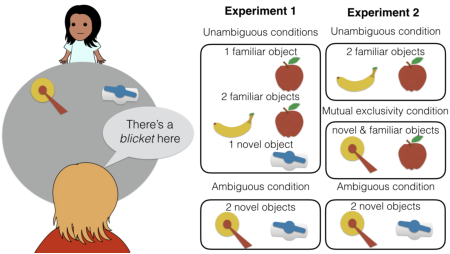
\includegraphics{figs/design-1} 

}

\caption[Study design for Experiments 1 and 2]{Study design for Experiments 1 and 2.}\label{fig:design}
\end{figure*}
\end{CodeChunk}

\section{Experiment 1}\label{experiment-1}

In Experiment 1, we examined whether children would reference a
speaker's face more often when there was referential ambiguity
associated with a label she produced. We were interested not only in
children's referencing of gaze direction during the labeling itself, but
referencing of the speaker after the labeling event while children made
a decision about which object was the intended referent. We predicted
that children would seek confirmation of the accuracy of their choice
from the speaker when they were uncertain, perhaps expecting an
emotional reaction or explicit approval, in addition to seeking gaze
direction information during labeling. We will refer to looks during and
after labeling as social referencing, as the looks could reflect
different types of information gathering.

We had children sit across from an experimenter who labeled an object on
the table between them (Figure \ref{fig:design}). Across trials, there
were either one or two objects, which were either familiar or unfamiliar
to the child. We expected children to be uncertain about the label's
referent only on trials with two unfamiliar objects. After labeling an
object, the experimenter asked the child to place the named object in a
bucket. We measured the number of times the child looked up to the
experimenter's face during four discreet phases of the trial: the
labeling event (\emph{label} phase), the sliding of the object(s) into
the child's reach (\emph{slide} phase), the time before the child
touched an object once they were within reach (\emph{planning} phase),
and the time between touching an object and dropping it in the bucket
(\emph{response} phase).

We predicted that children would look to the experimenter more often on
two-object novel trials compared to the other three trial types during
the labeling, planning, and response phases, which would indicate that
they recognized the need for disambiguating information. We did not
predict that children would look more for these trial types during the
slide phase, when they would likely be looking at the objects
themselves.

\subsection{Methods}\label{methods}

\subsubsection{Participants}\label{participants}

We recruited a planned sample of 80 children ages 2-5 years from the
Children's Discovery Museum in San Jose, California. The sample included
20 2-year-olds (mean age 31.71 months), 20 3-year-olds (mean age 42.65
months), 20 4-year-olds (mean age 55.85 months), and 20 5-year-olds
(mean age 65.11 months). An additional 20 children participated but were
removed from analyses because they heard English less than 75\% of the
time at home (\emph{n} = 10), because they were unable to complete at
least half of the trials in the task (\emph{n} = 4), because of parental
interference (\emph{n} = 1), or due to experimenter or technical errors
(\emph{n} = 5).

\subsubsection{Stimuli and Design}\label{stimuli-and-design}

In this task, children were presented with one or two objects, heard a
label, and were asked to put the labeled object in a bucket. Half of the
objects were selected to be familiar to children (e.g., a cow) and half
were selected to be novel (e.g., a nozzle). There were four trial types:
one-familiar, one-novel, two-familiar, and two-novel. There were three
trials of each type, for a total of twelve trials, and trial types were
presented sequentially in an order that was counterbalanced across
participants. The assignment of individual objects to trial types was
counterbalanced. On familiar trials, the familiar label for the target
object was used (e.g., ``cow''). On novel trials, a novel label was used
(e.g., ``dawnoo'').

The critical manipulation was of referential ambiguity; on one-familiar
and two-familiar trials, there was no referential ambiguity, as children
were expected to be certain about the objects and their labels.
Similarly, on one-novel trials, children were expected to be certain
about the label referent as there was only one option. However, on
two-novel trials, the referent was ambiguous, as the novel label could
apply to either novel object.

\subsubsection{Procedure}\label{procedure}

Throughout the study, the child sat at one end of a large circular
table, and the experimenter stood at the opposite end. Each trial of the
task proceeded as follows: the experimenter placed one or two objects on
the left and/or right sides of the table, out of reach of the child so
that the child could not interact with the toys during the labeling
event. For one-object trials, the location of the object (left or right)
alternated between trials. After placing the objects, the experimenter
said ``Hey look, there's a (target) here.'' The experimenter gazed at
the center of the table rather than the object she was labeling because
we wanted to preserve the referential ambiguity throughout the trial.
The experimenter waited approximately two seconds (based on a visual
metronome placed within view) before saying, ``Can you put the (target)
in the bucket?'' She then pushed the object(s) forward within reach of
the child, and placed a plastic bucket in the center of the table, also
within reach of the child. Prior to the twelve experimental trials,
there were two training trials: a one-familiar trial and a two-familiar
trial, to acquaint the child with the procedure. A camera placed to the
side of the experimenter captured the participant's face, so that
looking behavior could be coded from video.

\subsubsection{Coding procedure}\label{coding-procedure}

Videos were coded using DataVyu software (\url{http://datavyu.org}).
First, each trial was divided into four temporal phases: a \emph{label}
phase, which began at the utterance of the target label and ended when
the experimenter began to slide the objects, a \emph{slide} phase, which
encompassed the sliding of the objects into the child's reach, a
\emph{planning phase}, which began at the end of the slide and ended
when the child touched an object, and a \emph{response} phase, which
began when the child touched an object and ended when the child released
the object into the bucket. After onsets and offsets of these phases had
been coded, the coder recorded the number of looks the child made to the
experimenter's face during each phase. We opted to code the number of
looks rather than the duration of looks because we felt that looks from
the stimuli to the experimenter's face and vice versa might allow
children to integrate social and nonsocial information to solve the
problem of reference (refs), and might also be less sensitive to
individual differences in the duration of individual looks. A second
coder coded the number of looks for a quarter of the trials for each
participant to establish reliability. \emph{include reliability data
here}

\subsection{Results and Discussion}\label{results-and-discussion}

\begin{CodeChunk}
\begin{figure*}[h]

{\centering 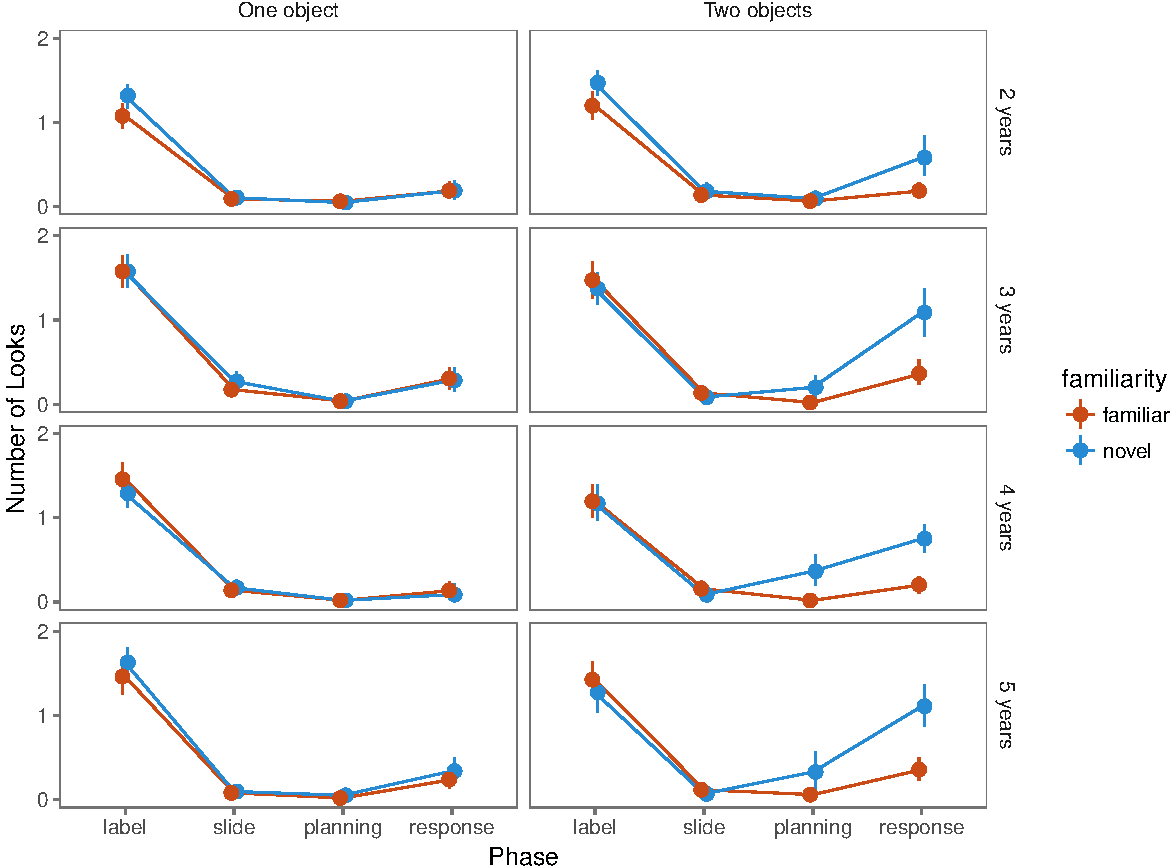
\includegraphics{figs/results_e1-1} 

}

\caption[Results of Experiment 1]{Results of Experiment 1. Number of looks to the experimenter across phases and conditions. Error bars are 95 percent confidence intervals.}\label{fig:results_e1}
\end{figure*}
\end{CodeChunk}

Descriptive results of Experiment 1 are presented in Figure
\ref{fig:results_e1}. To test our prediction that referential ambiguity
(i.e., having two novel objects) would produce more social referencing,
we fit mixed-effects linear regression models separately for each phase
with the following structure:
\texttt{number\ of\ looks\ \textasciitilde{}\ number\ of\ objects\ *\ familiarity\ *\ age\ in\ months\ +\ (number\ of\ objects\ +\ familiarity\ \textbar{}\ SID)}.
A single model with phase as a factor did not converge.

We did not find any main or interactive effects of number of objects,
familiarity, or age on number of looks during the label phase or the
slide phase. However, we found an interactive effect of number of
objects and familiarity during the planning (\(\beta\) = 0.21, \emph{p}
\textless{} .001) and response phases (\(\beta\) = 0.6, \emph{p}
\textless{} .001), such that 2-novel trials were associated with more
looking. There was no interaction with age in either
phase\footnote{Code and data available with full regression model results at https://github.com}.
In summary, children ages 2-5 looked to the experimenter more often when
planning and executing a response under uncertainty. These results
suggest that chidlren were aware that they did not have sufficient
knowledge to answer independently, and they attempted to resolve their
uncertainty using social referencing.

We did not find the expected effect of referential ambiguity in the
label phase. There are a number of reasons we might have observed this
null effect. One possibility is that children failed to predict that
they would need more information until later in the trial, when they
were actually faced with planning and executing a decision. Another
possibility is that children's looking was at ceiling during the
labeling phase, perhaps because children look at someone who is speaking
regardless of the need for referential disambiguation. A third
possibility is that this is an artifact of our design, in which the
experimenter gazed at the center of the table rather than the referent
of her label. Children may have realized that the experimenter's gaze
direction during labeling was not a source of disambiguating
information. Experiment 2 seeks to examine this possibility.

\section{Experiment 2}\label{experiment-2}

Experiment 2 was designed to replicate Experiment 1 and address the
possibility that the experimenter's gaze pattern during labeling had an
effect on children's social referencing. To test this possibility, we
manipulated the experimenter's gaze behavior between participants. For
half of the sample, the experimenter gazed at the center of the table
during labeling (i.e., reproducing Experiment 1), and for the remaining
half, the experimenter looked at the object she was referring to during
labeling. In Experiment 1, we did not observe an effect of age on
looking. Thus, we restricted the current sample to 3- and 4-year-olds.
Finally, since we did not observe any difference between the
one-familiar and one-novel trials, we eliminated single-object trials,
leaving the 2-familiar and 2-novel trials. In addition to these trials,
we added 1-novel-1-familiar trials to examine children's looking
patterns when 2 objects are present and an unfamiliar label are
produced, but the label referent can be deduced through the principle of
mutual exclusivity.

\subsection{Methods}\label{methods-1}

\subsubsection{Participants}\label{participants-1}

We recruited a planned sample of 80 children ages 3-4 years from the
Children's Discovery Museum in San Jose, California. The sample included
40 3-year-olds (mean age 42.89 months) and 40 4-year-olds (mean age
53.47 months). An additional 20 children participated but were removed
from analyses because they heard English less than 75\% of the time at
home (\emph{n} = 9), because they were unable to complete at least half
of the trials in the task (\emph{n} = 7), or due to experimenter or
technical errors (\emph{n} = 4).

\subsubsection{Stimuli and Design}\label{stimuli-and-design-1}

The stimuli and design were similar to Experiment 1, except that we
eliminated 1-object trials. Instead, we included three trial types:
2-familiar (``familiar''), 2-novel (``novel''), and 1-novel-1-familiar
(``mutual exclusivity''). There were four of each trial type, totaling
twelve trials. In addition, we manipulated the experimenter's gaze
behavior between participants. For half of the participants, she looked
at the center of the table on every trial; for the remaining half, she
looked at the object she referred to on every trial.

\subsubsection{Procedure}\label{procedure-1}

The procedure was identical to Experiment 1, except that there were
three practice trials rather than two, so that children could experience
every trial type.

\subsection{Results and Discussion}\label{results-and-discussion-1}

\begin{CodeChunk}
\begin{figure*}[h]

{\centering 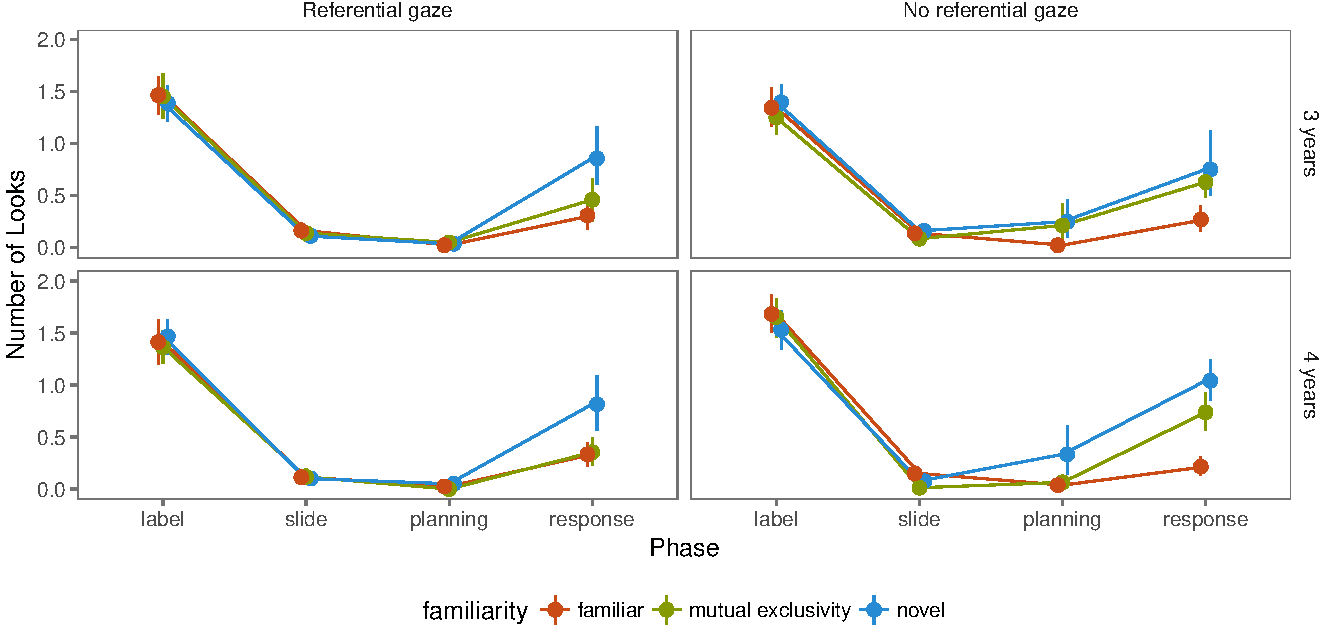
\includegraphics{figs/results_e2-1} 

}

\caption[Results of Experiment 2]{Results of Experiment 2. Number of looks to the experimenter across phases and conditions. Error bars are 95 percent confidence intervals.}\label{fig:results_e2}
\end{figure*}
\end{CodeChunk}

The descriptive results of Experiment 2 are presented in Figure
\ref{fig:results_e2}. To quantify the main and interactive effects of
familiarity, number of objects, gaze behavior, and age on social
referencing, we fit a mixed-effects linear regression model with the
following structure:
\texttt{number\ of\ looks\ \textasciitilde{}\ familiarity\ *\ age\ in\ months\ *\ gaze\ *\ phase\ +\ (familiarity\ \textbar{}\ SID)}.

As in Experiment 1, there was an interaction of phase with familiarity
such that the response phase of novel trials was associated with
significantly more looks (\(\beta\) = 0.51, \emph{p} \textless{} .001).
There was a three-way interaction of familiarity, gaze, and phase, such
that the response phase of mutual exclusivity trials in the no-gaze
condition was associated with more looks (\(\beta\) = 0.39, \emph{p}
\textless{} .01). Finally, we observed a four-way interaction such that
the response phase of novel trials in the gaze condition was associated
with more looking with increasing age (\(\beta\) = 0.06, \emph{p}
\textless{} .01).

Overall, these results replicate the finding from Experiment 1 that
children engage in more social referencing during the response phase
(i.e., when executing a decision about which item is being referred to)
when there is referential ambiguity because two novel objects are
present. However, we did not replicate the finding that children engaged
in more social referencing during the planning phase on novel trials. At
a descriptive level there was a trend for novel trials to be associated
with more looking in the no-gaze condition but not in the gaze
condition, perhaps because children were less uncertain after having
received helpful referential gaze during labeling.

In addition, we did not find selective social referencing during the
label phase, even when referential gaze was available. This rules out
the possibility that children were less selective during this phase
because they realized that gaze direction information was not available.
Instead, they might be at ceiling for looking (indeed, they do more
looking during this phase than the other three phases, regardless of
condition), or they may not recognize the additional need for
information in novel trials until they are faced with making a decision.

Interestingly, the three-way interaction of familiarity, gaze, and phase
showed that mutual exclusivity trials were associated with greater
looking during the response phase when the experimenter gazed at the
object she labeled compared to when she did not. This is intriguing
given that children should be able to solve mutual exclusivity trials
without gaze information. Instead, it seems that they remain somewhat
uncertain while executing a decision, but this uncertainty is resolved
if the experimenter gazes at the correct object during labeling.

Finally, the four-way interaction with age suggests that children
selectively reference social information in response to uncertainty to a
greater degree as they get older. This could be due to multiple factors;
on the one hand, they may more accurately monitor the need for
disambiguating information with development. On the other hand, they may
be more likely to recognize that social information can be a source of
disambiguation with age. Regardless, the interaction with age should be
interpreted with caution as we did not find any interaction with age in
Experiment 1.

\section{General Discussion}\label{general-discussion}

Preschoolers quickly learn new concepts, rules, and language, often with
minimal exposure (refs). They also actively explore and ask questions in
ways that seem targeted to maximize learning (Choinard, Schulz \&
Bonawitz). However, we still have an incomplete understanding of young
children's ability to monitor their own mental states, in particular,
their epistemic uncertainty. Do children monitor their own uncertainty
to guide information seeking behaviors, or are external features of the
environment sufficient to guide these behaviors (e.g., children might
ask for help with a complex looking toy in response to perceptual
features rather than epistemic states). Here, we examined a spontaneous
information-seeking behavior, social referencing, and its selectivity
with regard to epistemic uncertainty among preschool-aged children.
Specifically, we asked whether children would reference a social partner
more often when there was referential ambiguity in a label she produced,
and whether the amount of social referencing would reflect graded
uncertainty based on the availability of cues to reference.

We found strong evidence of selective social referencing under
referential ambiguity during the response phase of the trial, after
children had touched one of the objects but had not yet committed to it
by placing it in the bucket. In Experiment 1, we additionally found
evidence for selective social referencing earlier in the trial, after
the objects had been placed within reach but before the child touched
one of them, though this was not replicated in Experiment 2. Although we
cannot determine precisely what information children hoped to obtain
through these looks, we speculate that they may have expected
confirmation of the accuracy of their choice, either implicitly through
the adult's facial expressions, or through explicit feedback.

Importantly, we also found evidence for selectivity in social
referencing based on graded uncertainty. In Experiment 2, we manipulated
the amount of evidence available to children by including three trial
types: familiar trials in which children were familiar with the
label-object pairing and uncertainty should be low, novel trials in
which children were unfamiliar with the object-label pairing and
uncertainty should be high, and trials in which children could use
mutual exclusivity to discover the label-object pairing, but were not
previously familiar with the label or object. We also manipulated
whether or not gaze direction during labeling was useful; half of
participants had an experimenter who gazed at the object she labeled,
and half had one who gazed at neither object and was thus uninformative.

We found that children treated mutual exclusivity trials more like
familiar trials in terms of the amount of looking, but only when they
had received helpful gaze, suggesting that the combination of mutual
exclusivity cues and gaze direction cues were required for children to
feel confident about the object-label mapping. When mutual exclusivity
trials were not paired with helpful gaze, they were treated more like
novel trials. Importantly, useful gaze during labeling did not lessen
the amount of social referencing during the response phase for novel
trials, suggesting that gaze information alone was not sufficient to
reduce uncertainty. This means that children demonstrate uncertainty in
the presence of multiple objects and an unfamiliar label even when they
should be able to answer independently. It is possible that they remain
uncertain about a new label even after they have acquired it, if they
have only heard it once and not received confirmation of it's accuracy,
for example, through gaze monitoring.

On the other hand, we found no evidence for selectivity as the object
was being labeled, or as the objects were being slid into reach. One
interpretation of this pattern of results is that preschool-aged
children do not recognize the need for disambiguating information when a
referent is ambiguous until they are in the position of needing to make
a decision, at the end of the trial. However, another possibility is
that children spontaneously look at someone who is speaking regardless
of the need for disambiguating information, and additional looking on
top of this baseline was not needed or possible. A related possibility
is that the labeling phase of our task was too fast for children to
engage in extra looking on top of baseline in response to uncertainty.
Note that Vaish, Demir and Baldwin found that infants selectively
referenced a speaker during the labeling itself. However, their
procedure was different from the present study in that children were
holding one of the toys as the speaker produced a label. Thus,
referencing the speaker required disengaging from an interesting toy
that they were already attending to. This may have prevented ceiling
levels of looking and forced infants to be selective. A follow-up to the
present work that includes a greater trade-off in attentional
possibilities would help to distinguish among these possibilities.

Overall, these results confirm that preschool-aged children monitor
graded uncertainty in their knowledge and act on that uncertainty
through information-gathering behaviors. These findings contribute to an
emerging view of children's early learning as active and driven by
probabilistic evidence.

\section{Acknowledgements}\label{acknowledgements}

We thank Veronica Cristiano for assisting with data collection.

\section{References}\label{references}

\setlength{\parindent}{-0.1in} \setlength{\leftskip}{0.125in} \noindent

\end{document}
